%\title{Nyoka Sound Library Report}
\documentclass[letterpaper]{article}

\usepackage[english]{babel}
\usepackage[utf8x]{inputenc}
\usepackage{amsmath}
\usepackage{graphicx}
\usepackage[colorinlistoftodos]{todonotes}

\title{Universidad de Costa Rica \\ Escuela de Ingeniería Eléctrica \\ IE-217 Esctructuras abstractas de datos y algoritmos para ingeniería \\ Nyoka Sound Library Report}
\author{Arturo Apú Chinchilla B20386 \\ Guillermo Cornejo Suárez B22054 \\ José Johel Rodríguez Pineda B25706}

\begin{document}
\maketitle

\begin{center}
\rule{\textwidth}{0.8 pt} \\ [10 pt]
\end{center} 

\section{Introduction}

The developed project is a digital audio signal processing library. Digital signal processing (DSP) is the mathematical manipulation of an information signal to modify or improve it in some way. It is characterized by the representation of discrete time and discrete frequency by a sequence of numbers and the processing of these signals. This library works with sound signals, specifically mono-stereo files with ogg container and vorbis codec. 

\section{Background}
The earliest example of digital processing was probably in the 25th century BC. The Nile was the main source Egypt, however it's floods were a capricious meteorological phenomenon. The floods od the Nile were recorded by an array of measuring stations called "nilometers"; teh resulting data is considered a full-fledge digital signal defined on a time base of twelve months.\\
Analog signal processing has an important issue: analog recordings are not abstracs of the signal but the conversion of a physical phenomenom into another physical phenomenon. In a thermograph, for example, the temperature is converted into the amount of ink on the paper. Electronics did not change this thinking: an audio tape is obtained by converting a pressure wave into a electric current, the into a magnetic deflection. \\
Then, \textit{quantization} along with sampling was thought to be the way to obtain a fully digital signal: if a phenomenom is modeled as an analytical function, both the argument and the function's value are continuos variables;if it is known that that the mesures of the phenomenom have a fixed number of digits, the set of all possible measures is contable so it have been effectively mapped the function's values onto a set of integer numbers.\\
Digital signals provide us with a very usefull, simple and powerfull abstract representation of phenemonons. They can be reproduced exactly because they are a sequence of zeros and ones. They can also be manipulated easily. Since the signal is just a sequence of zeros and ones, and since a computer can do anything specifiable to such a sequence, a user do a great many things with digital signals.\\
Finally, digital processing allows the coexistence of standard processing with sophisticated decision logic; this enables the implementation of compression techniques and the inclusion of psychoperceptual models in order to match the compression strategy to the characteristics of the human visual or auditory system. 


\section{Development}
The functions supported in Nyoka Sound Library are the following:
\begin{enumerate}
\item \textbf{Decoder.} Decodes an ogg vorbis sound file into a real array.
\item \textbf{Encoder.} Encodes a real array into a ogg vorbis sound file.
\item \textbf{Fast Fourier transform.} Computes the one-dimensional discrete Fourier transform, which converts the decoded signal from time domain to frequency domain. 
\item \textbf{Inverse Fast Fourier transform.} Converts a signal in frequency domain to time domain computin the one-dimensional discrete inverse Fourier transform.
\item \textbf{Sine transform.} Using the fast Fourier transform, converts a signal from time domain to the frequency using sines only as a complete set of functions.
\item \textbf{Cosine transform.} Using the fast Fourier transform, converts a signal from time domain to the frequency using cosines only as a complete set of functions.
\item \textbf{Pitch filter.} Method for detecting pitched/unpitched sound. Tracks the pitch strength trace of the signal determining clusters of pitch and unpitched sound. The criterion used to determine the clusters is the
local maximization of the distance between the centroids.
\item \textbf{Low pass filter.} Passes low-frequency signals and reduces the amplitude of signals with frequencies higher than the cutoff frequency.
\item \textbf{High pass filter.} Passes high-frequency signals and reduces the amplitude of signals with frequencies lower than the cutoff frequency. 
\item \textbf{Band pass filter.} Passes frequencies within a certain range and attenuates frequencies outside that range.
\end{enumerate}

\subsection{Decoder and encoder}
Ogg Vorbis is a fully open, non-proprietary, patent-and-royalty-free, general-purpose compressed audio format for mid to high quality (8kHz-48.0kHz, 16+ bit, polyphonic) audio and music at fixed and variable bitrates from 16 to 128 kbps/channel. This library allows developing to obtain the total number of samples in a file. Also allows encoding a real array into a sound file. 

\subsection{Fast Fourier transform and inverse}
A process can be described in either the time domain or the frequency domain. In time domain by the values of $h(t)$ and in the frequency by it's amplitud as a functions of frequency $H(s)$. They are both representation of the same functions and are related to each other by the Fourier ecuations:
\begin{align}
	H(s)= \int\limits_{-\infty}^\infty h(t) e^{2\pi st} dt \\
    h(t)= \int\limits_{-\infty}^\infty H(s) e^{-2\pi st} ds
\end{align}
Now, the Fourier transform of a function with finite sample points is the aproximation of the previos equations by a discrete sum. It is called the \textbf{dicrete Fourier transform} of N points $h_k$:
\begin{align}
	H(s_n)=\int\limits_{-\infty}^\infty h(t) e^{2\pi s_n t} dt \approx \Delta \sum_{k=0}^{N-1} h_k e^{2\pi i k n /N} \\
    \rightarrow H_n=\sum_{k=0}^{N-1} h_k e^{2\pi i k n /N}
\end{align}
Similary, the discrete inverse Fourier transform is the following:
\begin{align}
	h_k= \frac{1}{N} 	\sum_{k=0}^{N-1} H_n e^{-2\pi i k n /N}
\end{align}
The methods used to compute de discrete Fourirer transform until 1960 showed that this transform is a $O(N^2)$ process; this is, in fact, amazingly immense. Danielson and Lanzcson rediscovered in 1942 a derivations of the algorithm latter called \textbf{fast Fourier transform}, that is in ther order of $O(N log_2 N)$ (independently discovered by Gauss in 1805). \\
The fast Fourier Transform's algorithm states that a transform length $N$ can be written as the summ of two length $N/2$ transforms, one with the odd-numbered points and the other with the even-numbered ones. This can be used recursively, the $N/2$ even-numbered transform can be reduced to a $N/4$ odd-numbered data and a $N/4$ even-numbered data. If $N$ is a power of 2, this can be continuosly applied until the data is subdivided to transforms of length one.\\ 
Bit reversal reordering is the methot used to figure out wich $n$ corresponds to a even or odd tranform. The algorithm combines adjacent pairs to get two-point transforms, and so on, until the first and second halves of the whole data set are combined into the final transform.\\
Then the final algorithm sorts the data into bit reverse order, then applies transforms of all de power 2 lengths until N, for each stage  two inner loops oscillate over the elements of each transform and the subtransforms alredy computed.

\subsection{Sine transform} 
The discrete sine transform expresses a finite sequence of data points in terms of a sum of sine functions oscillating at different frequencies. Fast Fourier transform uses both sines and cosines, but only half as many of each.\\
The sine transform is define as follows:
\begin{align}
F_k= \sum_{j=0}^{N-1}f_j \sin(\pi j k /N)	
\end{align}
With a bit of algebra it is easy to prove the following transform of a extended function:
\begin{align}
F_k=\sum_{j=0}^{2N-1}f_je^{2\pi i j k / 2N}= 2i\sum_{j=1}^{N-1}f_j \sin(\pi j k /N)	
\end{align}
Therefore, the sine transform may be obtained from the fast Fourier transform of  an extended function, up to a factor of $2i$. This method, however, introduces a factor of two inefficiency.	So, for the input data $f_j$ is necessary an auxiliar array $y_j$:
\begin{align}
y_j=\sin(j\pi /N)(f_j-f_{N-j})+\frac{1}{2}(f_j-f_{N-j})
\end{align}
Applying fast Fourier transform to $y_j$ and after a bit of algebra, the real and imaginary part are given by:
\begin{align}
R_k=\sum_{j=0}^{N-1}y_j\cos(2\pi jk/N)=F_{2k+1}-F_{2k-1}\\
I_k=\sum_{j=0}^{N-1}y_j\sin(2\pi jk/N)=F_{2k}
\end{align}
The sine transform is its own inverse, if applied twice the return array is the original one multiplied by a factor  of $N/2$.

\subsection{Cosine transform}
The discrete cosine transform expresses a finite sequence of data points in terms of a sum of cosine functions oscillating at different frequencies.
The cosine transform is define as follows:
\begin{align}
F_k= \sum_{j=0}^{N-1}f_j \cos(\pi j k /N)	
\end{align}
Again, a extended fast Fourier transform (this time of length $N+1$) obtains the cosine transform:
\begin{align}
F_k= \frac{1}{2}(f_0+(-1)^kf_N)+\sum_{j=1}^{N-1}f_j \cos(\pi j k /N)	
\end{align}
As expected, besides the entrance $f_j$ another auxiliar function $y_j$ is nedeed.
\begin{align}
y_j=-\sin(j\pi /N)(f_j-f_{N-j})+\frac{1}{2}(f_j+f_{N-j})
\end{align}
This time:
\begin{align}
R_k=\sum_{j=0}^{N-1}y_j\cos(2\pi jk/N)=F_{2k}\\
I_k=\sum_{j=0}^{N-1}y_j\sin(2\pi jk/N)=F_{2k+1}-F_{2k-1}
\end{align}

\subsection{Pitch filter}
Algorithm designed by Dr. Arturo Camacho. The method tracks the pitch strength trace of a signal, determining clusters of pitch and unpitched sound. The criterion used to determine the clusters is the local maximization of the distance between the centroids. \\
Pitch is a perceptual phenomenon that allows ordering sounds in a musical scale, it directly depends on the amount of vibrations per second of the sound. However, not all sounds have pitch. This classification of sounds into pitched and unpitched is useful in applications like music transcription and speech coding.\\
This filter estimates the pitch strength of a signal using the SWIPE algorithm, for doing pitched/unpitched detection. This algorrithm estimates the pitch strength at a discrete time as the spectral similarity between the signal and a sawtooth waveform with missing non-prime harmonics and same pitch as the signal.\\
The filter determines, at every instant of time $n$, the assigment of classes to samples in the neighrborhood of $n$ using the maximations if the distance between the centroids of the classes as optimization criterion.\\
To determine the optimal class assignment for each sample $n'$ in the neighborhood of $n$ the filter first weights the sample using a Hand window of size $2N+1$ centered at n:
\begin{align}
w_n=(n'-n)=1+\cos\left(\frac{\pi(n'-n)}{N+1}\right)
\end{align}
The assigment of claasses is represented by $\mu(n')$; $\mu(n')=0$ means that the signal at $n'$ is unpitchetd and $\mu(n')=1$ means that the signal at $n'$ is pitchetd.\\
Then, the centroid of the pitched class is determined by:
\begin{align}
c_1(n,\mu,N)=\frac{\sum_{n'=-N}^N \mu(n'-n)s(n'+n)w_N(n')}{\sum_{n'=-N}^N \mu(n'+n)w_N(n')}
\end{align}
And the centroid of the unpitched class:
\begin{align}
c_0(n,\mu,N)=\frac{\sum_{n'=-N}^N (1-\mu(n'-n))s(n'+n)w_N(n')}{\sum_{n'=-N}^N (1-\mu(n'-n)) w_N(n')}
\end{align}
Finally, the class membership of the signal at time $n$:
\begin{align}
m(n)=\left(\frac{s(n)-c_o}{c_i-c_o}\right)
\end{align}
$N$ is defined recursively from $1$ until the size of the pitch stregth trace is reached increasing  its values by  a factor of $2^{1/4}$. The algorithm stops when $\mu$ reaches a fixed point or  after 100 iterations.
\subsection{Low pass, High pass and Band pass filters}
A low-pass passes low-frequency signals and reduces the amplitude of signals with frequencies higher than a cutoff frequency.\\
A high-pass passes high-frequency signals but reduces the amplitud of signals with frequencies lower than a cutoff frequency.\\
A band-pass combines a high and low pass filter. 

\section{Installing}
\subsection{Requierements}
To plot you need to install gnuplot. For ubuntu/debian:
\begin{center}
\$ sudo apt-get install gnuplot\\
\end{center}
To decode or encode the library needs the ogg and vorbis external library. Both are include in external\_libraries directory. To install ogg, open a terminal, enter to nyonka\_snd\_lib/external\_libraries/libogg-version and make:
\begin{center}
	\$ ./configure\\
	\$ make\\
	\$ sudo make install
\end{center}
\subsection{Compiling}
A compiling script can be found in main directory. To run it you first need to change it's premissions in order to make it executable. This can be done by opening the library directory in a terminal and typing:
\begin{center}
	\$ chmod u+x compile.sh
\end{center}
Next, to compile the whole library you can make:
\begin{center}
	\$ ./compile.sh
\end{center}
To compile you need to have installed in you sistem the requirement listed above, the g++ compiler and the pkg-config utility. To do so you can open a terminal and type (assuming you are using debian or a derivate):
\begin{center}
	\$ sudo apt-get install g++\\
	\$ sudo apt-get install pkg-config	
\end{center}	
Pkg-config is an utility to make easier finding headers and .so (shared objects) of libraries while compiling. Although Nyoka\_snd\_lib do no install anything in your sistems it reliesin other libraries and needs this utility to find them. 

\section{Using}
You use the library as follows. See Figure 1.
\begin{figure}
\centering
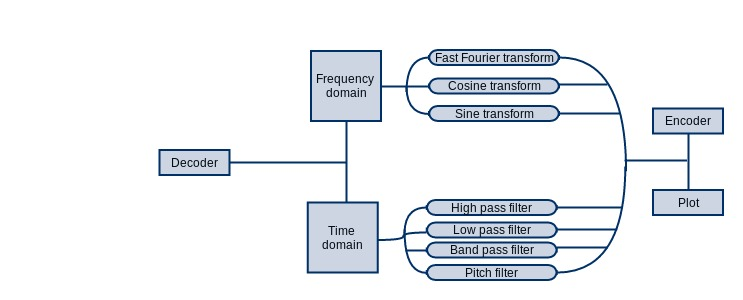
\includegraphics[width=1\textwidth]{diagrama_nyoka__1_.jpg}
\caption{\label{fig:libraryFlowDiagram}Nyoka Sound Library Design.}
\end{figure}

	First, you may decode a ogg vorbis sound file usinde Decode, then you can choose to apply a frequency domain or time domain function. Fast Fourier transform, cosine transform and sine transform are the frequency {}domain functions and all the filters are time domain ones. After applying this function, you may either encode the array back to a sound file or plot the result.\\
	Nyoka sound library is formed up of binary compiled objects,
which can be found in build directory. To use the library you need to
include the right headers in you source code and, while compiling your
program, you need to link with the corresponding object file. 
	You can look in examples directory to check the implementation
and compiling process. Next is a brief explanation:

	Take for example the decoder.cpp program, which is in examples
directory. First you find the include statments. In line 5 we included
the header <plot.hh> to be able to plot sound in time a frequency domain.
Once you set the right include statments in your programs you must
tell the compiler where to find them, in this case the header files 
are in include directory, then using g++ (if you are using another
compiler you should read it's documentation about including headers)
\begin{center}
	\$ g++ -c -I../include decoder.cpp
\end{center}
The above command tells g++ to compile (-c) decoder.cpp, and let it knows
where to find the requiere headers, -I stands for include and next is 
the relative path. 
	Once compiled you need to create a executable file. 
\begin{center}
	\$ g++ -o decoder.exe decoder.o ../build/plot.o \$(VORBIS)
\end{center}
This indicates g++ to create an executable output file (-o decoder.exe)
using the compiled source from decoder.o (the program we just compiled above)
and ../build/plot.o, a compiled object from Nyoka\_snd\_lib. The \$(VORBIS)
stuff is just a variable, while running it is replaced by it's content,
in this case the first line of examples/makefile.\\
	Now you have an executable file that integrates the compiled
source of your program and Nyoka sound library.\\
Those are the tools, now have fun.

\section{Bibliography}
\begin{enumerate}
\item Prando, P., Vetterli, M. (2008). \textit{Signal Processing for communications}. Paris and Grandvaux.
\item S. A. Martucci.(1994). \textit{Symmetric convolution and the discrete sine and cosine transforms}. IEEE Trans. Sig. Processing. 
\item Camacho, A. (2008). \textit{Detections of pitched/unpitched sound using pitch strength  clustering}. ISMIR - Section 4c - Automatic Music Analysis and Transcription.
\item Brassard, G., Bratley, P. (1998). \textit{Fundamentos de Algoritmia}.  Départament d'informatique et de recherche opérationelle, Universuté de Montréal. Pretice Hall.
\end{enumerate}

\end{document}